%%%%%%%%%%%%%%%%%%%%%%%%%%%%%%%%%%%%%%%%%%%%%%%%%%%%%%%%%%%%%%%%%%%%%%%%%%%%%%%%
\chapter{Детали реализации}
%%%%%%%%%%%%%%%%%%%%%%%%%%%%%%%%%%%%%%%%%%%%%%%%%%%%%%%%%%%%%%%%%%%%%%%%%%%%%%%%

\nomenclature{PSI}{Program Structure Index}
\nomenclature{AST}{Abstract Syntax Tree}

% ИСходный код может быть найден там-то и там-то. Зафиксировать версию компилятора.

\section{Внутреннее устройство компилятора языка програмиирования Kotlin}

Работу компилятора языка программирования Kotlin можно разделить на два этапа: анализ исходных текстов программы и генерация байт-кода. 

\begin{figure}[htbp]
    \centering
    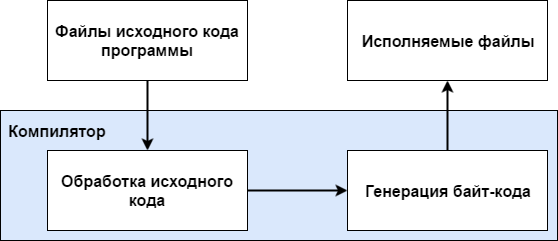
\includegraphics[width=\textwidth]{resources/06/01_compiler_scheme.png}
    \caption{Этапы работы компилятора языка программирования Kotlin}
    \label{fig05:compiler-scheme}
\end{figure}

На первом этапе сначала происходит синтаксический разбор текста исходного кода программы, в результате чего формируется абстрактное синтаксическое дерево, описывающие программу. Затем на основе полученной модели строится \emph{индекс структуры программы} (\emph{program structure index} --- \emph{PSI}), который содержит уже не только синтаксическую, но также и семантическую информацию о структуре программы. Перечислим основные элементы, из которых состоит PSI модель программы, и их роли:
\begin{itemize}
    \item Абстрактное синтаксическое дерево играет роль источника синтаксической информации в модели.
    \item Декларации являются точкой доступа к семантической информации о программе. Всякая сущность, которая имеет объявление внутри программы (класс, метод и т.д.), имеет соответствующую декларацию в PSI модели.
    \item Ссылки позволяют связывать узлы абстрактного семантического дерева и декларации. Таким образом, например, все использования класса в программе на синтаксическом уровне могут быть связаны с единственной декларацией, соответствующей этому классу. 
\end{itemize}
Строго говоря, PSI модель программы является намного более сложной структурой, нежели описано выше и используется в семействе интегрированных сред разработки, разрабатываемых компанией JetBrains, как средство рефлективного представления исходного кода программы. В рамках компилятора, однако, данное средство используется весьма ограничено и по большей части на стадии разбора исходного текста программы. После построения PSI модели происходит преобразование ее в набор \emph{дескрипторов}, с которыми удобнее работать на стадии генерации байт-кода. Не все дескрипторы должны предоставлять какую-либо синтаксическую информацию, что позволяет иметь синтетические программные сущности, которые не представлены в исходном коде в явном виде. В то же время, всякий дескриптор суть есть семантика соответствующих элементов. Основное отличие дескрипторов от PSI элементов заключается в том, что дескрипторы связаны общей системой типов, которая строится по мере анализа программы. Таким образом, именно на этапе анализа программы происходит \emph{разрешение} (\emph{resolution}) типов и проверяется корректность их использования. 

\todo{Сказать, что часто используется, когда вычисление значения и его использование отделены друг от друга} Одним из центральных элементов всего процесса компиляции является экземпляр типа \lstinline{BindingTrace}. Он важен здесь по двум причинам. Во-первых, интерфейс \lstinline{BindingTrace} расширяет интерфейс \lstinline{DiagnosticSink}, который предоставляет методы по сбору диагностических сообщений, что позволяет организовать обратную связь с пользователем компилятора. Во-вторых, \lstinline{BindingTrace} позволяет сохранять любую информацию на стадии анализа для дальнейшего ее переиспользования на этапе генерации байт-кода. Хранение информации организовано в виде пар ключ-значение, где ключ состоит из двух частей: идентификатора среза (который также хранит информацию о типах второй части ключа и значения) и обычного ключа, как он понимается в структуре данных \lstinline{Map}. Все идентификаторы срезов объявлены в интерфейсе \lstinline{BindingContext}, который также предоставляет некоторые операции по работе со срезами информации и сбору диагностических сообщений. Основным отличие \lstinline{BindingContext} от \lstinline{BindingTrace} заключается в том, что, в случае использования первого, данные доступны только для чтения, в то время как, в \lstinline{BindingTrace} также заложена возможность записи данных. По этой причине \lstinline{BindingContext}, как правило, реализуется как анонимный класс внутри конкретной реализации \lstinline{BindingTrace}, большая часть логики которого состоит в делегации вызовов вышестоящему экземпляру \lstinline{BindingTrace}.   

\begin{figure}[htbp]
    \centering
    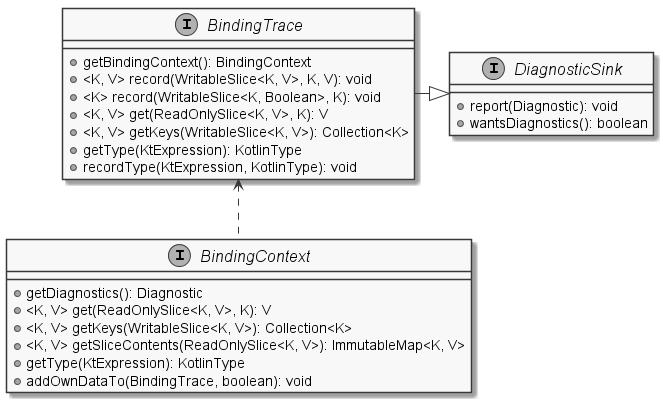
\includegraphics[width=\textwidth]{resources/06/04_binding_context.png}
    \caption{Стурктура интерфейса \lstinline{BindingTrace}}
    \label{fig05:binding-trace-scheme}
\end{figure}

Описание \lstinline{BindingContext} насчитывает порядка шестидесяти объявлений идентификаторов срезов данных. Большинство из них описывают срезы, которые хранят соответствие деклараций и дескрипторов, однако есть и те, которые предназначены для хранения информации о типах, потоке данных переменных, областях видимости и т.д. Вся эта информация используется, во-первых, для выявления ошибок в программном коде и, во-вторых, для генерации байт-кода.

\begin{figure}[htbp]
    \centering
    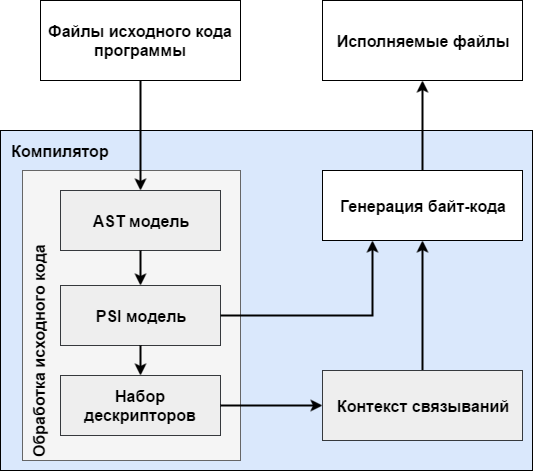
\includegraphics[width=\textwidth]{resources/06/04_compiler_flow_diagram.png}
    \caption{Стурктура интерфейса \lstinline{BindingTrace}}
    \label{fig05:binding-trace-scheme}
\end{figure}

После анализа файлов исходного кода в случае, если не было выявлено каких-либо критических ошибок, начинается этап генерации байт-кода. Данный процесс организован последовательно для всех файлов исходного кода. В случае возникновения исключения в процессе обработки конкретного файла, происходит его перехват и обработка, которая, как правило, заключается в передаче исключения на уровень выше в стеке вызовов или в выводе информации об исключении. Если исключение не было передано дальше, процесс генерации байт-кода продолжится со следующего файла, в противном случае прерывается весь процесс компиляции.  

В пределах конкретного файла объявляется следующий порядок обработки элементов: сначала генерируется байт-код для классов, интерфейсов и объектов, объявленных в данном файле, а затем для всех других определений, которые встречаются в файле (функции, свойства и пр.). Одним из основных классов здесь является \lstinline{MemberCodegen}: именно в нем определяются базовые методы, отвечающие за генерацию членов классов, а также порядок обработки самого класса (интерфейса, объекта). 

\begin{figure}[htbp]
    \centering
    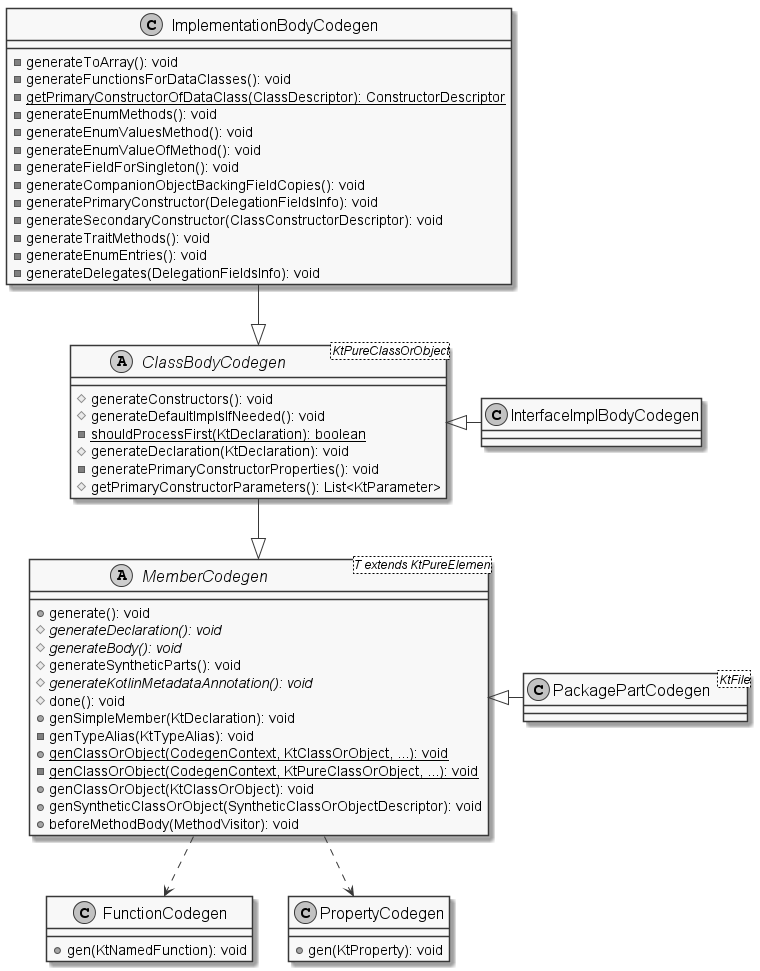
\includegraphics[width=\textwidth]{resources/06/06_member_codegen.png}
    \caption{Стурктура интерфейса \lstinline{BindingTrace}}
    \label{fig05:binding-trace-scheme}
\end{figure}

Порядок определяется вне зависимости от того, является ли обрабатываемая сущность классом, интерфейсом или объектом, следующим образом:
\begin{enumerate}
    \item Генерация объявления сущности.
    \item Генерация тела сущности. На данном этапе генерируется байт-код для всех сущностей, объявленных внутри рассматриваемой. Это могут быть как свойства и функции, так и другие классы, объекты и т.д. В случае, если на этом шаге встречается класс, интерфейс или объект, порядок их обработки также соответствует настоящему списку. 
    \item Генерация синтетических частей сущности. Под синтетическими частями здесь понимается часть функциональности сущности, которая абсолютно корректна с точки зрения использования в контексте рассматриваемой сущности, однако не объявляются нигде в исходном коде программы. Сюда, например, относятся специальные методы \lstinline{values} и \lstinline{valueOf}, относящиеся к \emph{перечислениям} (\emph{enum}), а также все необходимые методы для \emph{классов данных} (\emph{data classes}).  
    \item В случае необходимости (определяется настройками процесса компиляции) генерируются аннотации метаданных.
\end{enumerate}
Для всякого типа генерируемой сущности в компиляторе представлена подходящая реализация \lstinline{MemberCodegen}, в которой определяется каким именно образом будут обрабатываться объявление, тело и синтетические части класса. Свойства и функции, в свою очередь, с точки зрения пользователя \lstinline{MemberCodegen} генерируются для всех типов сущностей одинаково.

\section{Разработка демонстрационной версии механизма классов типов в языке программирования Kotlin}

При разработке демонстрационной версии приоритетной была поставлена задача реализации и интеграции всех алгоритмов, необходимых для обеспечения существенной части функциональности механизма классов типов. На данном этапе реализации также допустимы некоторые расхождения с концепцией, представленной в разделе \ref{sct:overview-conclusion}. Тем не менее, демонстрационная версия должна удовлетворять всем требованиям, представленным в разделе \ref{sct:problem-constraints}. Такой подход позволяет получить рабочую версию компилятора, которая допускает использование классов типов, однако, возможно, обладает некоторыми изъянами, касающимися в основном выразительной части разработанного механизма. 

Сначала зафиксируем форму представления всех элементов, необходимых для использования классов типов. Возьмем за основу пример, представленный в тексте программы \ref{lst:concept-example}, и упростим его. Прежде всего перечислим основные возможности, которые необходимо предоставить пользователю для полноценного использования классов типов:
\begin{enumerate}
    \item Объявить класс типов.
    \item Объявить экземпляр класса типов.
    \item Объявить принадлежность произвольной типовой переменной функции некоторому классу типов.
    \item Вызвать произвольную функцию, принадлежащую экземпляру класса типов для типовой переменной с соответствующим ограничением.   
\end{enumerate}
Заметим, что наибольшую сложность здесь вызывает последний пункт, поскольку на данном этапе не совсем понятно, как это должно выглядеть с точки зрения пользователя. Кроме того, введение ограничения на принадлежность типовой переменной классу типов, в соответствии с предложенной концепцией решения (и, как следствие, подходом, который используется в языке программирования Haskell), \todo{ссылка на пример, который показывает, что это должен быть именно аргумент.} подразумевает введение неявных переменных. То есть помимо того, что необходимо подставить подходящую реализацию класса типа, используемого в некоторой функции, в точку вызова этой функции, также следует создать видимость того, что аргумент-словарь, соответствующий классу типов, присутствует в данной функции и именно он должен использоваться в качестве носителя реализаций функции, принадлежащих этому классу типов. Таким образом, трудности, связанные с реализацией последних двух элементов списка, описанного выше, связаны одной общей проблемой, а именно отсутствием в области видимости функции, использующей класс типов, ссылки на словарь \todo{их? надо где-то сказать, что рассмотрим для одного} соответствующего класса типов. Наиболее простым способом предоставить пользователю такую ссылку представляется ее явное объявление в сигнатуре функции. Этого можно достичь несколькими способами (например, можно использовать все те же аннотации). Напомним, однако, что на данном этапе было решено сосредоточиться на реализации и интеграции алгоритмов, обеспечивающих хотя бы базовую функциональность механизма классов типов. По этой причине было решено использовать наиболее простой из доступных вариантов, которым \todo{надо бы хоть как-то мотивировать простоту} оказался подход, заключающийся в следующем:
\begin{enumerate} 
    \item Введем аннотацию \lstinline{@TypeClassDisctionary}, область допустимого использования которой ограничена аргументами функций. 
    \item В случае, когда аргумент некоторой функции имеет тип, соответствующий классу типов, и помечен аннотацией \lstinline{@TypeClassDisctionary}, в точке вызова такой функции запрещается указывать данный аргумент явно. Вместо этого пользователь должен расчитывать на то, что все такие аргументы будут подставлены компилятором автоматически. 
    \item В случае, если какие-либо условия из пункта $2$ нарушены, генерируются диагностические сообщения об ошибках.
\end{enumerate}
\todo{сказать, что ограничение на типовую переменную преобразуется} Заметим, что строгий запрет на явное указание аргументов вызова функции, которые должны быть подставлены компилятором самостоятельно, является существенным в контексте описанного выше подхода по той простой причине, что в противном случае невозможно будет определить правильный порядок аргументов вызова. Кроме того, такой запрет позволяет избежать неоднозначности. Стоит отметим, однако, что эту проблему можно решить и другими способами (например, определением порядка объявления явных и неявных аргументов), однако, поскольку все рассмотренные решения были приблизительно одинаково сложны с точки зрения реализации, было выбрано наиболее гибкое из них. Предлагаемое допущение позволяет существенно упростить задачу. Де-факто, для реализации демонстрационной версии достаточно модифицировать компилятор таким образом, чтобы:
\begin{itemize}
    \item Всякий раз, когда встречается аргумент, помеченный аннотацией \lstinline{@TypeClassDisctionary} и тип которого соответствует классу типов, организуется поиск подходящего экземпляра класса типов с учетом доступной информации о значениях типовых переменных. Если подходящий экземпляр не найден, генерируется диагностической сообщение об ошибке. В противном случае результат поиска сохраняется.
    \item Всякий раз при обработке вызова функции, список аргументов вызова формируется с учетом дополнительной информации об уже найденных для данного вызова экземплярах классов типов. Если при этом какой-то из аргументов, помеченных аннотацией \lstinline{@TypeClassDisctionary} уже указан, генерируется диагностическое сообщение об ошибке.
\end{itemize}
Таким образом, на уровне представления в исходном коде программы предлагаемый подход аналогичен \todo{подобрать более подходящее слово} псевдореализации классов типов в языке программирования Haskell (см. текст программы \ref{lst:haskell-example-pseudo-impl}) с той лишь только разницей, что здесь запрещается явное указание аргументов-словарей в точке вызова всякой функции. Нечто подобное существует и в языке программирования Scala и называется \emph{неявными параметрами} (\emph{implicit parameters}). 

\lstinputlisting[
    label={lst:scala-implicit-parameters},
    caption={Пример использования неявных параметров в Scala},
    style={scala}
]
{resources/06/07_scala_implicit_parameters}

Использование механизма неявных параметров позволяет объявить для функции список дополнительных неявных аргументов, которые не указываются в точке вызова и подставляются компилятором, исходя из значений типовых переменных.

\todo{Перенести все это в обзорную часть?} Единственный вопрос, который до сих пор не был рассмотрен, касается стратегии создания словаря, соответствующего экземпляру класса типов, в точке вызова. Понятно, что в точке вызова функции, использующей классы типов, при применении рассматриваемого подхода не представляется возможным указать аргументы, которые необходимо передать в конструктор соответствующего экземпляра класса типов. Таким образом, на этапе подстановки аргументов в вызов такой функции, необходимо либо уже иметь экземпляр объекта, соответствующий экземпляру класса типов, либо наперед знать о, конкретной \emph{функции-поставщике}, которая способна такой экземпляр предоставить и которая при этом не принимает аргументов. В случае использования функции-поставщика сразу же возникает вопрос о сохранении состояния используемого экземпляра класса типов как объекта. Если состояние экземпляра класса типов изменяется в процессе работы, необходимо определить, в какой области его использования такой экземпляр должен быть представлен в единственном виде. Даже если доступ к экземпляру класса типов осуществляется через уже готовую ссылку (фактически, посредством переменной), необходимо среди всех подходящих ссылок выбрать правильную. \todo{Подумать об оформлении в замечания}

Заметим, что наличие более чем одного источника одного или нескольких типов, способного предоставлять экземпляры класса типа, для отдельно взятого экземпляра класса типов, предполагает наличие некоторого механизма, который будет выбирать единственный источник. Такой механизм, очевидно, с точки зрения функциональности имеет много общего с механизмом неявных определений, представленном в языке программирования Scala. Напомним, что неявные определения в Scala вносят определенную долю неоднозначности, которая может затруднить или исказить понимание сути кода с точки зрения стороннего пользователя. Кроме того, благодаря механизму  допущение о наличии более чем одного источника экземпляров классов типов в языке программирования Kotlin способно неявным образом нарушить требование о \todo{дать название требованиям, чтобы ссылать без помех} единственности экземпляра класса типов для всякой пары класса типов и типа даже в случае, когда источник экземпляра класса типов указывается явно в точке вызова. Это становится возможным, благодаря тому, как устроена работа с \emph{вариантными} (\emph{variancve}) типами в Kotlin. Рассмотрим пример, представленный в листинге \ref{lst:single-instance-violation}. Прежде всего определим семантику аннотаций, используемых в этом примере:
\begin{itemize}
    \item Семантика аннотации \lstinline{@TypeClass} идентична тому, как она приводится в разделе \ref{sct:concept-annotations-processing}. \todo{зафиксировать эту семантику где-то. фиксировать каждый раз? ...} 
    \item Аннотация \lstinline{@TypeClassSupplier} значит, что под ней приводится определение сущности (свойства, функции, классы специального вида и т.д.), которая тем или иным образом (посредством вызова или обращения, например) способна предоставить экземпляр класса типов.     
\end{itemize}

\lstinputlisting[
    label={lst:single-instance-violation},
    caption={Пример кода, допускающего нарушение требования о единственности экземпляра класса типов},
    style={kotlin}
]
{resources/06/09_single_instance_violation}

Таким образом, в примере, представленном в листинге \ref{lst:single-instance-violation} существует два источника, способных предоставить экземпляра класса типов для класса типов \lstinline{Default} и типа \lstinline{Number}. Пусть существуют две точки вызова произвольных функций (возможно, одинаковых), каждая из которых использует класс типов \lstinline{Default}. Пусть также, в одной из таких точек вызова в качестве источника экземпляра класса типов был выбран объект \lstinlint{NumberDefault}, а в другом --- функция \lstinline{getDefaultForNumber}. Тогда в две эти точки вызова будут подставлены разные реализации интерфейса \lstinline{Default}, каждая из которых является экземпляром класса типов \lstinline{Default} для типа \lstinline{Number}. Здесь можно сказать, что уже из самих объявлений экземпляров классов типов следует нарушение требования единственности на основании того, что экземпляр класса типов \lstinline{Default} для типа \lstinline{Number} с точки зрения системы типов может быть использован вместо экземпляра для типа \lstinline{Double}. Это утверждение легко опровергнуть, поскольку, несмотря на наличие более чем одного подходящего экземпляра, в такой ситуации компилятор может быть запрограммирован таким образом, чтобы выбор был сделан в сторону наиболее точного по типу экземпляра. В свою очередь, в примере, представленном в листинге \ref{lst:single-instance-violation}, реализация такого подхода не представляется возможным.   

Учитывая приведенные выше доводы, было решено ввести ограничение на единственность \todo{как-то формализовать этот термин что ли?} источника, предоставляющего доступ к конкретному экземпляру класса типов. Вопрос о том, какой вид источников предпочтителен, остается открытым. С одной стороны использование функций-поставщиков представляется более гибким, поскольку позволяет отделить конфигурацию объектов от их использования (что, строго говоря, является одним из основных архитектурных принципов в объектно-ориентированном программировании). Альтернативный подход заключается в том, чтобы для каждого экземпляра класса типов была определенная переменная, которая хранит единственный экземпляр типа и которая используется всюду для доступа к экземпляру класса типов. Такой подход равносилен использованию шаблона проектирования \todo{кавычки?} одиночка (singleton) по отношению ко всем экземплярам классов типов. Использование второй стратегии, конечно, обязывает пользователя разрабатывать экземпляры классов типов таким образом, чтобы они были безопасны для использования несколькими потоками исполнения и, к тому же, быть более осторожным при введении состояния объекта, однако, в то же время представляется более простой для реализации. Именно поэтому на этапе разработки демонстрационной версии было решено осуществлять доступ к экземплярам классов типов вторым способом. Стоит отметить, что язык программирования Kotlin по умолчанию поддерживает шаблон проектирования \todo{?} одиночка. Для этого в язык был введен новый для Java вид объявлений --- объекты. Объекты по сути являются классами, для которых компилятор автоматически генерирует статическое поле для хранения единственного экземпляра и инициализирует его правильным образом. Таким образом, можно сделать предлагаемый подход более наглядным и еще более простым с точки зрения реализации, если ограничить способы определения экземпляров классов типов только лишь объектами. В рамках разработки демонстрационной версии было решено использовать данное ограничение. 

\lstinputlisting[
    label={lst:demo-usage-example},
    caption={Пример использования классов типов в демонстрационной версии механизма классов типов},
    style={kotlin}
]
{resources/06/08_demo_usage_example}

\todo{перечислить минусы?}

\section{Реализация демонстрационной версии механизма классов типов в языке программирования Kotlin}

% На первый взгляд, реализация всех алгоритмов, необходимых для поддержания функционирования демонстрационной версии механизма классов типов, не представляет большой сложности: достаточно иметь доступ к экземпляру класса \lstinline{BindingTrace} вместе с некоторыми вспомогательными классами и функциями. Наибольшие сложности возникли с тем, чтобы найти наиболее подходящее место для интеграции всех этих алгоритмов.
%С точки зрения внутреннего устройства компилятора процесс функционирования базовой версии механизма классов типов был организован следующим образом:
Процесс обработки объявлений классов типов, их экземпляров и функций, использующих классы типы, в базовой версии механизма классов типов был реализован следующим образом:  
\begin{enumerate}
    \item Каждый раз, когда встречается определение объекта, который является \todo{где-то сказать про это} прямым наследником типа, объявление которого помечено аннотацией \lstinline{@TypeClass}, извлекается множество значений типовых переменных, присущих этому типу. Затем дескрипторы этого объекта и объявления его базового типа вместо со значениями всех значимых типовых переменных сохраняются. 
    \item В месте разрешения вызова функции для всякого аргумента, помеченного аннотацией \lstinline{@TypeClassDictionary}, вычисляется его тип с учетом значений типовых переменных, доступных в области видимости рассматриваемого вызова, и все известные типы экземпляров классов типов проверяются на соответствие этому вычисленному типу, после чего извлекается определение объекта, соответствующее найденному типу экземпляра класса типов. Найденное таким образом объявление, вызов и соответствующий аргумент, сохраняются. В случае, если подходящего экземпляра класса типов не было найдено, генерируется сообщение об ошибке, а значение рассматриваемого аргумента принимается равным \lstinline{null}. 
    \item Перед генерацией аргументов вызова на стеке вместе с объявленными аргументами извлекаются также значения всех неявных аргументов, вычисленных для данного вызова. Все аргументы объединяются в единый список в порядке, соответствующем порядку объявления аргументов в определении функции, который в дальнейшем используется по стандартному сценарию.    
\end{enumerate}   
Рассмотрим каждый из этих этапов более подробно.

Всякий дескриптор класса владеет информацией о собственном базовом типе (включая, значения типовых переменных) и его дескрипторе. Таким образом, первый этап описанного выше процесса теоретически может быть реализован сразу после создания дескриптора класса. Основная логика, связанная с управлением процессом создания дескрипторов, расположена в классе \lstinline{LazyTopDownAnalyzer}. 

\begin{figure}[htbp]
    \centering
    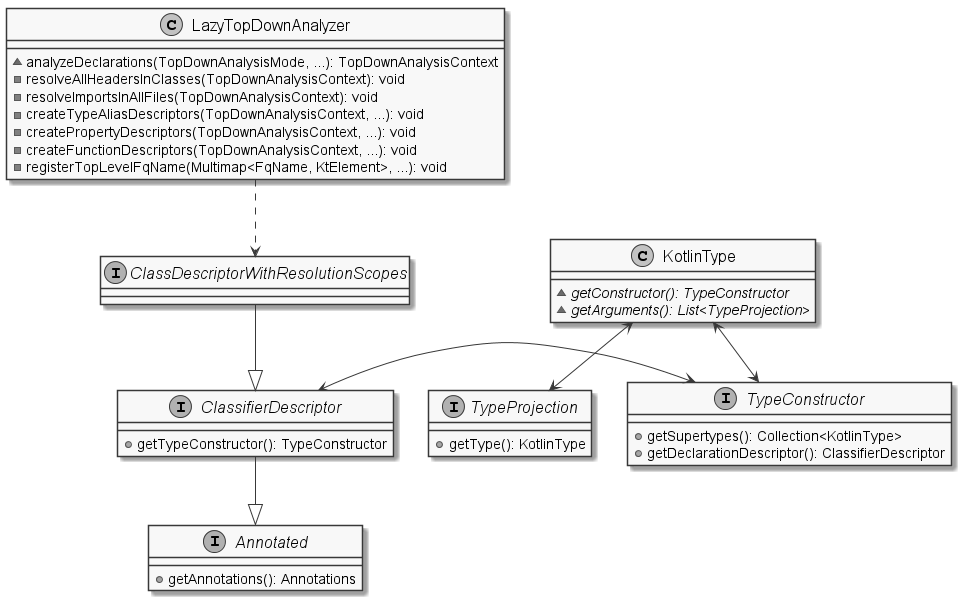
\includegraphics[width=\textwidth]{resources/06/12_class_descriptor.png}
    \caption{Стурктура класса \lstinline{LazyTopDownAnalyzer}}
    \label{fig:lazy-top-down-analyzer}
\end{figure}

Здесь организован рекурсивный перебор всех деклараций, находящихся в компилируемых файлах. Дескрипторы классов создаются прямо в процессе перебора ленивым образом, в то время как все остальные декларации просто запоминаются и преобразуются в дескрипторы уже после просмотра предоставленных файлов. Стоит обратить внимание на то, что большинство компонент деклараций, соответствующих объявлениям классов в исходном коде программы, также создаются ленивым образом. Ленивые вычисления здесь играют важную роль, поскольку позволяют не только игнорировать порядок обхода файлов компилятором, но, к тому же, разрешать некоторые циклические зависимости в исходном коде. В некоторых случаях преждевременное обращение к определенным составляющим дескриптора класса может привести к исключению на этапе компиляции. Таким образом, обработку информации об экземплярах классов типов целесообразно проводить уже после того, как все компоненты дескрипторов классов могут быть вычислены. Это становится возможным в самом \lstinline{LazyTopDownAnalyzer} после того, как будет вызван метод \lstinline{resolveAllHeadersInClasses}. Более того, внутри этого метода компоненты всех найденных дескрипторов классов вычисляются и, соответственно, дальнейшие манипуляции с дескрипторами не нарушают неявных контрактов, связанных с ленивыми вычислениями. Хранить информацию об экземплярах классов типов было решено внутри контекста связываний. Такое решение можно объяснить тем, что экземпляр одного из типов \lstinline{BindingTrace} или \lstinline{BindingContext} доступен практически на любом этапе компиляции программы, что позволяет обеспечить доступ к информации о классах типов там, где это будет необходимо. Идентификатор соответствующего среза данных был размещен внутри объявления \lstinline{BindingContext} и выглядит как показано в листинге \ref{lst:demo-type-class-slice}.

%В первую очередь заметим, что \todo{просто было решено?} наиболее удобным способом сохранения информации о классах типов и их экземплярах, является использование экземпляра класса \lstinline{BindingTrace}. Такое положение вещей объясняется тем, что экземпляр одного из типов \lstinline{BindingTrace} или \lstinline{BindingContext}, как правило, доступен практически на всех этапах компиляции программы, что позволяет обеспечить доступ к данной информации там, где это будет необходимо. Альтернативный вариант заключается в том, чтобы хранить всю информацию о доступных экземплярах класса типов прямо внутри экземпляра дескриптора, соответствующего описанию класса типа. Однако в этом случае внутри дескриптора класса, соответствующего классу типов, появлялась бы циклическая зависимость, поскольку всякий дескриптор класса по умолчанию уже хранит (пусть и в неявном виде) ссылку на дескриптор базового типа. Таким образом, в первую очередь необходимо создать подходящий идентификатор среза данных, в котором будет храниться вся необходимая информация. Объявление этого среза выглядит как показано в листинге \ref{lst:demo-type-class-slice} и было размещено внутри определения класса \lstinline{BindingContext}.

\lstinputlisting[
    label={lst:demo-type-class-slice},
    caption={Объявление идентификатора среза данных, предназначенного для хранения классов типов и их экземпляров вместе со значениями типовых переменных, присущих классу типов, в демо версии механизма классов типов},
    style={kotlin}
]
{resources/06/10_demo_type_class_slice}

%Для того, чтобы осуществить запись данных в этот срез, необходимо иметь ссылки на дескриптор, соответствующий экземпляру класса, его базовый класс и значения всех типовых переменных, присущих этому базовому классу, а также экземпляр класса \lstinline{BindingTrace}. Все данные, необходимая для формирования записи, могут быть извлечены из любого экземпляра класса \lstinline{ClassDescriptor}. Создание дескрипторов классов, как и всех остальных типов дескрипторов (функции, свойств и т.д.), происходит на этапе анализа исходного кода программы. Большая часть логики, связанной с определением порядка создания и обработки дескрипторов в штатном режиме работы компилятора, расположена в классе \lstinline{LazyTopDownAnalyzer}. Здесь организован рекурсивный перебор всех деклараций, находящихся в компилируемых файлах. Дескрипторы классов создаются прямо в процессе перебора ленивым образом, в то время как все остальные декларации просто запоминаются и преобразуются в дескрипторы уже после просмотра имеющихся файлов. В классе \lstinline{BindingContext}, помимо прочего, присутствует объявление идентификатора среза данных \lstinline{CLASS}, который предназначен для хранения соответствия между дескрипторами и декларациями классов. При более подробном рассмотрении процесса создания дескрипторов классов, можно определить места записи данного среза данных, которыми оказались, конструкторы классов \lstinline{LazyJavaClassDescriptor} и \lstinline{LazyClassDescriptor}. Таким образом, на первый взгляд, запись в срез \lstinline{TYPECLASS_IMPLEMENTATIONS} может быть организована прямо внутри конструктора дескриптора класса. На деле же, это не совсем так, по крайне мере в общем случае, поскольку почти все компоненты внутри \lstinline{LazyJavaClassDescriptor} и \lstinline{LazyClassDescriptor} создаются ленивым образом. Ленивое вычисление этих компонент играет очень важную роль, поскольку для корректной работы многих из них необходима информация о компонентах, которые еще не были обработаны компилятором. В то же время, для определения того, является ли рассматриваемый класс экземпляром класса типов, необходимо вычислить точное значение его базового класса, то есть необходимо запустить соответствующий процесс вычислений, который может завершиться некорректно и привести в непредвиденным ошибкам. По этой причине было решено осуществлять запись в срез \lstinline{TYPECLASS_IMPLEMENTATIONS} там, где по крайней мере все классы и типы уже вычислены. Подходящим место записи, например, является место создания всех дескрипторов сущностей, отличных от классов. Именно там и было организовано распознавание и запись экземпляров классов типов.  

Теперь, когда информация о классах типов и их экземплярах сохраняется в контексте связываний, перейдем к рассмотрению процессов обработки и генерации вызовов функций. За генерацию байт-кода вызова функции отвечает класс \lstinline{ExpressionCodegen}. Сам класс реализует интерфейс посетителя в шаблоне проектирования \todo{кавычки?} посетитель, в котором элементами являются декларации. Таким образом, \lstinline{ExpressionCodegen} обрабатывает не только вызовы, но также и все другие существующие виды деклараций. Аргументы вызова извлекаются из экземпляра класса \lstinline{ResolvedCall}, который, в свою очередь, достается из специального среза данных в контексте связываний.     

\begin{figure}[htbp]
    \centering
    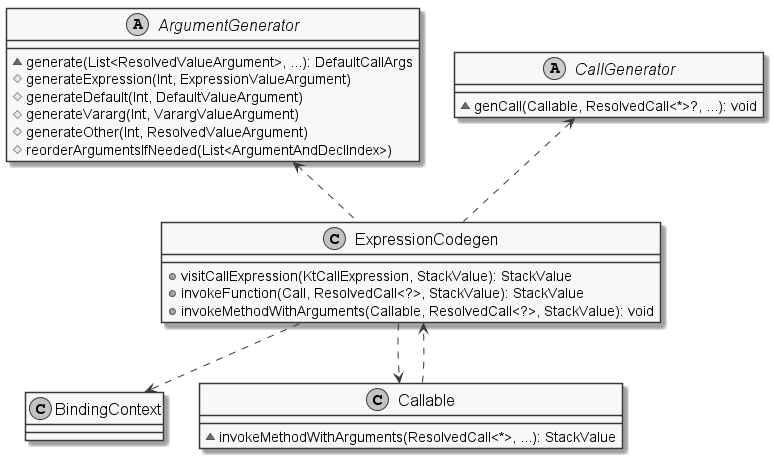
\includegraphics[width=\textwidth]{resources/06/11_expression_codegen.png}
    \caption{Стурктура класса \lstinline{ExpressionCodegen}}
    \label{fig:expression-codegen}
\end{figure}

Экземпляры класса \lstinline{ResolvedCall} создаются и сохраняются на этапе поиска функции-кандидата, вызов которой обрабатывается. За формирование списка параметров вызова отвечает класс \lstinline{CandidateResolver}. Процесс обработки аргументов вызова устроен следующим образом:
\begin{enumerate}
    \item Проверка фиктивности дескриптора функции-кандидата. Если дескриптор фиктивный, то никаких дальнейших проверок не производится, при этом считается, что процесс разрешения этого кандидата завершен успешно.  
    \item Проверка области видимости класса, членом которого является рассматриваемый кандидат. 
    \item В зависимости от режима проверки типов либо происходит сопоставления значений аргументов вызова параметрам рассматриваемой функции-кандидата, либо производится проверка возвращаемого типа функции. В первом случае в экземпляр класса \lstinline{ResolvedCall} добавляется информация о соответствии аргументов функции-кандидата и значениях, указанных в точке вызова, а также для каждого известного аргумента записывается статус, который отражает состояние аргумента в системе типов функции кандидата.  
    \item Проверка типов ресиверов (receiver) функции.
    \item Если значения типовых переменных указаны явно в точке вызова, то строится соответствующий им подстановщик типов, который затем используется для присвоения значений типовым переменным внутри дескриптора кандидата.
    \item Проверка значений аргументов функции в точке вызова. Если значения типовых переменных указаны явно в точке вызова, то значения аргументов проверяются на соответствие полученной системе типов. В противном случае, типы параметров функции в точке вызова вычисляются, при этом в процессе вычисления типов строится соответствующая им система типов. Вызов в этом случае считается корректным если полученная система типов не имеет противоречий.      
    \item Проверка того, что рассматриваемая функция-кандидат не является абстрактной. Также проверяются некоторые специальные случаи использования суперклассов. 
    \item Проверка корректности использования вызова в случае, если рассматриваемый кандидат является конструктором псевдонима типов (type alias). 
\end{enumerate}

\begin{figure}[htbp]
    \centering
    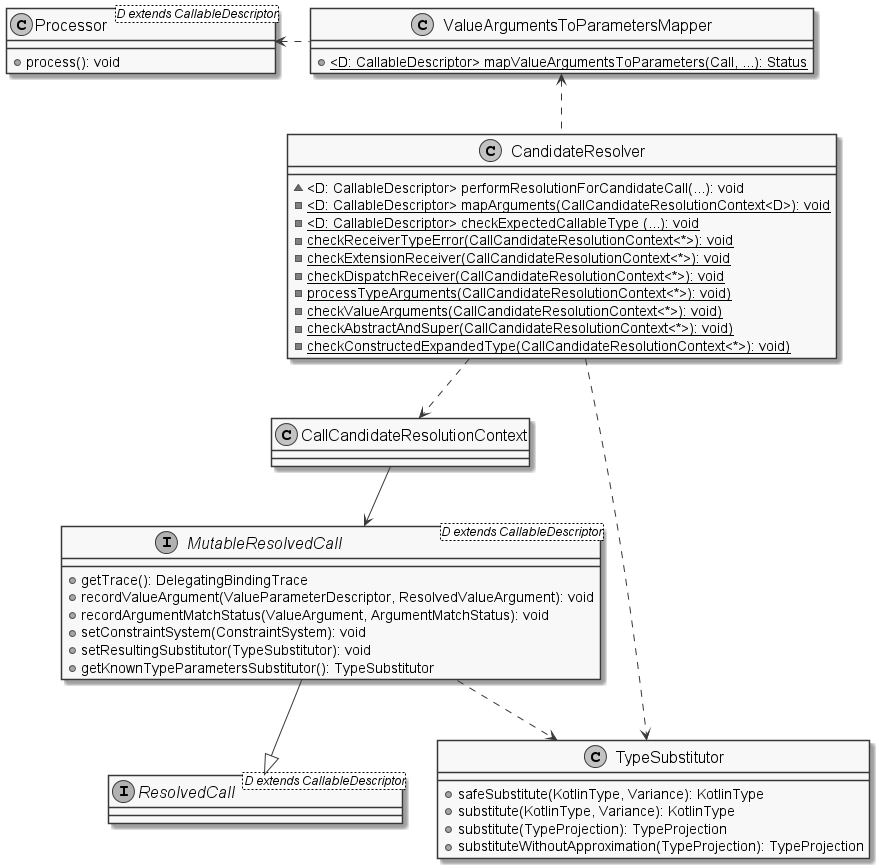
\includegraphics[width=\textwidth]{resources/06/13_candidate_resolver.png}
    \caption{Стурктура класса \lstinline{CandidateResolver}}
    \label{fig:candidate-resolver}
\end{figure}

Напомним, что в соответствии с предложенным подходом, неявные аргументы не указываются в точке вызова. Таким образом, ошибка компиляции в описанном выше процессе, возникает уже на третьем шаге. Для разрешения этой проблемы в процессе обхода аргументов функции-кандидата производится проверка на присутствие аннотации \lstinline{@TypeCLassDictionary}. В случае, если рассматриваемый аргумент помечен такой аннотацией, его значение не извлекается из списка параметров, указанного в точке вызова, но принимается равным \lstinline{null}. Помимо этого, в соответствие такому аргументу ставится специальный статус, который позднее позволит отличить аргументы, значения которых должны быть вычислены компилятором самостоятельно, от тех, которые указываются пользователем. Теперь необходимо определить точку, в которой в экземпляр \lstinline{ResolvedCall} получает информацию о значениях типовых переменных. Вся информация, касающаяся данного аспекта вызова объединена в единый класс \lstinline{TypeSubstitutor} (подстановщик типов), обработка которого происходит в методе \lstinline{setResultingSubstitutor} класса \lstinline{ResolvedCall}. В случае, если значения типовых переменных указаны явно в точке вызова, соответствующий подстановщик типов строится и передается на обработку уже на шестом этапе описанного выше процесса. В противном случае, подстановщик типов будет построен позже (за это отвечает класс \lstinline{GenericCandidateResolver}), однако обрабатываться он будет таким же образом. В процессе обработки подстановщика типов в \lstinline{ResolvedCall} все известные до этого параметры создаются заново с учетом новой информации о значениях типовых переменных. Кроме того, внутри экземпляра класса \lstinline{ResolvedCall} есть доступ к экземпляру класса \lstinline{BindingTrace}. Таким образом, здесь не представляет большой сложности выбрать подходящий экземпляр класса типов: достаточно извлечь список параметров типа аргумента, играющего роль словаря класса типов, и, используя этот список и дескриптор объявления типа как ключ, запросить все доступные экземпляры класса типа из известного среза данных.    

На этом реализацию демонстрационной версии механизма классов типов можно считать завершенной. 

\section{Модификация прототипа механизма классов типов}

%В данном разделе будут рассмотрены модификации демонстрационной версии механизма классов типов, которые были интегрированы в компилятор языка программирования Kotlin в рамках данной работы. 
Одним из существенных недостатков прототипа механизма классов типов является то, что описанная реализация может вычислить подходящий экземпляр класса типов в точке вызова только в том случае, если значения типовых переменных принимают значения реальных типов. Другими словами, существующий подход не способен корректно обработать ситуацию, в которой вызов функции, использующей классы типов, расположен внутри другой функции, использующей тот же класс типов и предполагается, что соответствующие экземпляры классов типов должны быть идентичны (то есть представлены ссылкой на один и тот же экземпляр класса). В этом случае подходящий экземпляр класса типов может быть извлечен из области видимости, соответствующей функции-обертке рассматриваемого вызова. Задачу можно упростить, приняв во внимание тот факт, что переменная-словарь класса типов может встречаться только в списке аргументов функции. Заметим также, что даже в случае, когда экземпляр класса типов может быть вычислен, основываясь на значениях типовых переменных, однако в функции-обертке присутствует подходящий аргумент-словарь, также целесообразно использовать уже имеющийся экземпляр. Таким образом, на этапе сопоставления значений аргументов вызова параметрам рассматриваемой функции-кандидата необходимо интегрировать следующий алгоритм:
\begin{enumerate}
    \item Определить вышестоящую декларацию и, если эта декларация соответствует определению функции, перейти к следующему шагу. В противном случае настоящий алгоритм завершается.
    \item Проверить каждый аргумент функции-обертки, помеченный аннотацией \lstinline{@TypeClassDictionary}, на равенство типов с каким-либо параметром, соответствующим классу типов, в рассматриваемом вызове.
    \item Для всякой пары, найденной на предыдущем шаге, значение параметра в точке вызова принимается равным соответствующему аргументу функции-обертки.
\end{enumerate} 
С технической точки зрения для извлечения вышестоящего дескриптора можно воспользоваться экземпляром класса \lstinline{BindingContext}: сначала извлекается из специального среза данных извлекается область видимости, доступная в точке вызова, а затем берется ее владелец. Проверка равенства типов осуществляется путем сравнения конструкторов этих типов (\lstinline{TypeConstructor}).  